\documentclass[12pt, a4paper]{article}

% ─── Packages ────────────────────────────────────────────────────────────────
\usepackage[top=2.5cm, bottom=2.5cm, left=2.8cm, right=2.8cm]{geometry}
\usepackage{graphicx}
\usepackage{booktabs}
\usepackage{array}
\usepackage{xcolor}
\usepackage{listings}
\usepackage{caption}
\usepackage{subcaption}
\usepackage{amsmath}
\usepackage{hyperref}
\usepackage{fancyhdr}
\usepackage{titlesec}
\usepackage{parskip}
\usepackage{microtype}
\usepackage{enumitem}
\usepackage{mdframed}
\usepackage{tikz}
\usepackage{colortbl}

% ─── Colors ──────────────────────────────────────────────────────────────────
\definecolor{alexblue}{RGB}{0, 56, 101}
\definecolor{accentblue}{RGB}{30, 100, 200}
\definecolor{lightgray}{RGB}{245, 245, 248}
\definecolor{codebg}{RGB}{28, 32, 40}
\definecolor{codegreen}{RGB}{80, 200, 120}
\definecolor{codepurple}{RGB}{180, 130, 255}
\definecolor{codeyellow}{RGB}{255, 215, 90}
\definecolor{codecyan}{RGB}{90, 210, 240}
\definecolor{codewhite}{RGB}{230, 230, 230}
\definecolor{tableheader}{RGB}{0, 56, 101}

% ─── Hyperref Setup ──────────────────────────────────────────────────────────
\hypersetup{
    colorlinks=true,
    linkcolor=accentblue,
    urlcolor=accentblue,
    citecolor=accentblue,
    pdftitle={GPU Matrix Operations Report},
    pdfauthor={Alexandria University}
}

% ─── Section Formatting ──────────────────────────────────────────────────────
\titleformat{\section}
  {\Large\bfseries\color{alexblue}}
  {\thesection.}{0.6em}{}[\color{alexblue}\titlerule]

\titleformat{\subsection}
  {\large\bfseries\color{accentblue}}
  {\thesubsection.}{0.5em}{}

\titlespacing{\section}{0pt}{18pt}{8pt}
\titlespacing{\subsection}{0pt}{12pt}{4pt}

% ─── Header / Footer ─────────────────────────────────────────────────────────
\pagestyle{fancy}
\fancyhf{}
\fancyfoot[C]{\small\thepage}
\renewcommand{\headrulewidth}{0pt}

% ─── Code Listing Style ──────────────────────────────────────────────────────
\lstdefinestyle{pythonstyle}{
    backgroundcolor=\color{codebg},
    basicstyle=\ttfamily\footnotesize\color{codewhite},
    keywordstyle=\color{codepurple}\bfseries,
    stringstyle=\color{codegreen},
    commentstyle=\color{gray}\itshape,
    numberstyle=\tiny\color{gray},
    numbers=left,
    numbersep=10pt,
    breaklines=true,
    showstringspaces=false,
    frame=none,
    xleftmargin=16pt,
    xrightmargin=4pt,
    aboveskip=6pt,
    belowskip=6pt,
    tabsize=4,
    morekeywords={import, as, def, for, in, return, True, False},
    literate=
        {0}{{\textcolor{codeyellow}{0}}}{1}
        {1}{{\textcolor{codeyellow}{1}}}{1}
        {2}{{\textcolor{codeyellow}{2}}}{1}
        {3}{{\textcolor{codeyellow}{3}}}{1}
        {4}{{\textcolor{codeyellow}{4}}}{1}
        {5}{{\textcolor{codeyellow}{5}}}{1}
        {6}{{\textcolor{codeyellow}{6}}}{1}
        {7}{{\textcolor{codeyellow}{7}}}{1}
        {8}{{\textcolor{codeyellow}{8}}}{1}
        {9}{{\textcolor{codeyellow}{9}}}{1},
}

\lstset{style=pythonstyle}

% ─── Custom Box ──────────────────────────────────────────────────────────────
\newmdenv[
  linecolor=accentblue,
  linewidth=1.2pt,
  backgroundcolor=lightgray,
  roundcorner=4pt,
  innerleftmargin=10pt,
  innerrightmargin=10pt,
  innertopmargin=8pt,
  innerbottommargin=8pt,
  skipabove=8pt,
  skipbelow=8pt
]{infobox}

% ═════════════════════════════════════════════════════════════════════════════
\begin{document}

% ─── Title Page ──────────────────────────────────────────────────────────────
\begin{titlepage}
\thispagestyle{empty}

\begin{center}

\vspace*{0.5cm}

% Top rule
{\color{alexblue}\rule{\linewidth}{2pt}}
\vspace{0.3cm}

{\color{alexblue}\large\textsc{Alexandria University --- Faculty of Engineering}}\\[0.15cm]
{\color{gray}\large Department of Computer Engineering}

\vspace{0.3cm}
{\color{alexblue}\rule{\linewidth}{0.5pt}}

\vspace{1.8cm}

{\color{alexblue}\fontsize{26}{32}\selectfont\bfseries
Using GPU in Matrix Operations}

\vspace{0.6cm}

\vspace{1.5cm}

% Decorative block

\begin{tikzpicture}
  \fill[alexblue!10, rounded corners=6pt] (0,0) rectangle (10,1.2);
  \draw[alexblue, line width=1pt, rounded corners=6pt] (0,0) rectangle (10,1.2);
  \node at (5, 0.6) {%
    \large\color{alexblue}
    \textbf{CPU} \quad vs \quad \textbf{GPU}
  };
\end{tikzpicture}

\vspace{2cm}

\begin{tabular}{rl}
  \color{gray}\textbf{Students:}  & \color{alexblue} Samaa Ibrahim El-Hakmy \quad \texttt{22010820} \\[4pt]
                                  & \color{alexblue} Nour-Eldin Akram Elsayed \quad \texttt{22011309} \\[4pt]
\end{tabular}

\vfill

{\color{alexblue}\rule{\linewidth}{0.5pt}}
\vspace{0.2cm}
{\color{gray}\small Alexandria University, Faculty of Engineering --- Spring 2026}
{\color{alexblue}\rule{\linewidth}{2pt}}

\end{center}
\end{titlepage}

% ═════════════════════════════════════════════════════════════════════════════
\section{Introduction}

Modern computing workloads---especially in machine learning, scientific simulation, and computer vision---are dominated by large-scale linear algebra. Matrix multiplication in particular is an $\mathcal{O}(n^3)$ operation whose cost grows rapidly with size. Graphics Processing Units (GPUs) offer massively parallel execution and high memory bandwidth that can dramatically reduce this cost compared to a traditional Central Processing Unit (CPU).

This lab explores that gap concretely. We implement the computation

\[
  D = A \times B \times C + A
\]

where $A, B, C \in \mathbb{R}^{n \times n}$, benchmark it with \textbf{NumPy} (CPU) and \textbf{CuPy} (GPU/CUDA) across nine matrix sizes from $128 \times 128$ to $10{,}000 \times 10{,}000$, and quantify the resulting speedup.

% ═════════════════════════════════════════════════════════════════════════════
\section{Methodology}

\subsection{Libraries}

\begin{itemize}[leftmargin=1.4em, itemsep=3pt]
  \item \textbf{NumPy 1.x} --- the standard Python array library, executing on a single CPU core using BLAS routines.
  \item \textbf{CuPy} --- a NumPy-compatible library that dispatches operations to an NVIDIA GPU via CUDA.  CuPy's \texttt{@} operator maps directly to \texttt{cuBLAS} \texttt{SGEMM}.
\end{itemize}

\subsection{Benchmarking Protocol}

\begin{infobox}
For each matrix size $n \in \{128, 256, 512, 1024, 1536, 2048, 4000, 8000, 10000\}$:
\begin{enumerate}[leftmargin=1.4em, itemsep=2pt]
  \item Allocate fresh random matrices $A, B, C$ of shape $n \times n$.
  \item Execute $D = A \times B \times C + A$ and record wall-clock time.
  \item Repeat 10 times; report the \textbf{mean} elapsed time.
  \item GPU timing uses \texttt{cp.cuda.Event} for device-accurate measurement.
\end{enumerate}
\end{infobox}

\clearpage
% ═════════════════════════════════════════════════════════════════════════════
\section{Implementation}

\subsection{Full Source Code}

\begin{lstlisting}[language=Python, caption={Complete benchmarking script}]
import numpy as np
import cupy as cp
import time
import matplotlib.pyplot as plt

SIZES   = [128, 256, 512, 1024, 1536, 2048, 4000, 8000, 10000]
REPEATS = 10

def benchmark_cpu(n):
    times = []
    for _ in range(REPEATS):
        A = np.random.rand(n, n)
        B = np.random.rand(n, n)
        C = np.random.rand(n, n)
        start = time.perf_counter()
        D = A @ B @ C + A
        end   = time.perf_counter()
        times.append(end - start)
    return np.mean(times)

def benchmark_gpu(n):
    times = []
    for _ in range(REPEATS):
        A = cp.random.rand(n, n, dtype=cp.float32)
        B = cp.random.rand(n, n, dtype=cp.float32)
        C = cp.random.rand(n, n, dtype=cp.float32)

        start = cp.cuda.Event()
        stop  = cp.cuda.Event()
        start.record()
        D = A @ B @ C + A
        stop.record()
        stop.synchronize()

        gpu_time_ms = cp.cuda.get_elapsed_time(start, stop)
        times.append(gpu_time_ms / 1000.0)

        del A, B, C, D
        cp.get_default_memory_pool().free_all_blocks()
    return np.mean(times)
\end{lstlisting}

\clearpage
\subsection{Key Design Decisions}

\begin{itemize}[leftmargin=1.4em, itemsep=3pt]
  \item \textbf{CUDA Events for GPU timing.} \texttt{time.perf\_counter()} measures host-side wall time which may not capture asynchronous GPU execution.  CUDA events are placed directly on the GPU stream, giving accurate device-side elapsed time.
  \item \textbf{Memory pool reset.} CuPy uses a memory pool by default.  Calling \texttt{free\_all\_blocks()} after each trial prevents cached blocks from flattering later allocations and ensures fair per-trial measurement.
  \item \textbf{Averaging over 10 runs.} A single run is noisy due to OS scheduling, cache warm-up, and CUDA JIT compilation on the first call.  The mean of 10 trials yields a stable estimate.
\end{itemize}

% ═════════════════════════════════════════════════════════════════════════════
\section{Results}

\subsection{Raw Benchmark Data}

\begin{table}[h!]
\centering
\caption{Benchmark results for all tested matrix sizes}
\vspace{4pt}
\begin{tabular}{
  >{\centering\arraybackslash}m{2.4cm}
  >{\centering\arraybackslash}m{3cm}
  >{\centering\arraybackslash}m{3cm}
  >{\centering\arraybackslash}m{2.8cm}
}
\toprule
\rowcolor{tableheader}
\color{white}\textbf{Matrix Size} &
\color{white}\textbf{CPU Time (s)} &
\color{white}\textbf{GPU Time (s)} &
\color{white}\textbf{Speedup} \\
\midrule
$128 \times 128$     & 0.000486  & 0.005921  & 0.08$\times$ \\
\rowcolor{lightgray}
$256 \times 256$     & 0.003224  & 0.000113  & 28.48$\times$ \\
$512 \times 512$     & 0.004777  & 0.000319  & 14.99$\times$ \\
\rowcolor{lightgray}
$1024 \times 1024$   & 0.022501  & 0.001095  & 20.55$\times$ \\
$1536 \times 1536$   & 0.067980  & 0.003041  & 22.35$\times$ \\
\rowcolor{lightgray}
$2048 \times 2048$   & 0.150264  & 0.007616  & 19.73$\times$ \\
$4000 \times 4000$   & 1.073150  & 0.063962  & 16.78$\times$ \\
\rowcolor{lightgray}
$8000 \times 8000$   & 7.704448  & 0.577311  & 13.35$\times$ \\
$10000 \times 10000$ & 15.117782 & 0.721720  & 20.95$\times$ \\
\bottomrule
\end{tabular}
\label{tab:results}
\end{table}


\begin{figure}[h!]
  \centering
  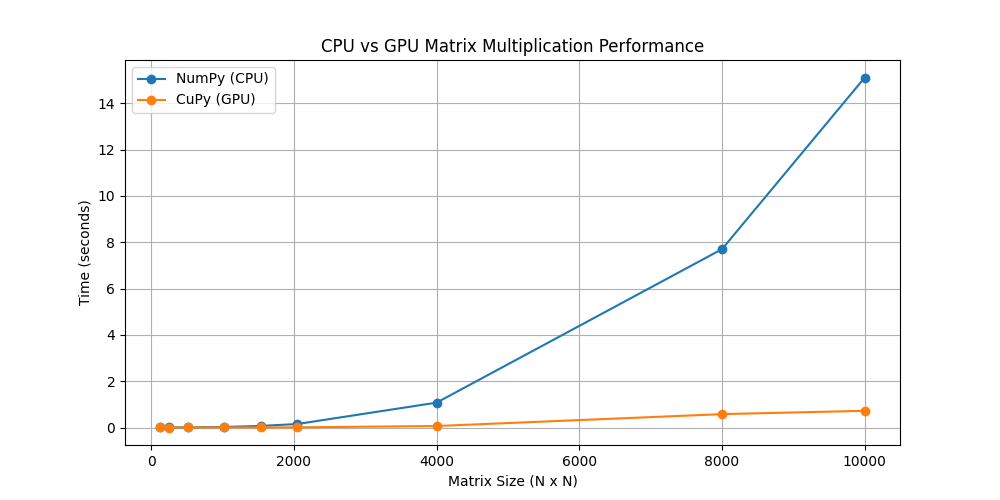
\includegraphics[width=0.92\textwidth]{cpu_gpu_comparison.png}
  \caption{Absolute execution time for NumPy (CPU) vs.\ CuPy (GPU) as a function of matrix size. The CPU curve grows steeply beyond $n = 4000$, while the GPU curve remains nearly flat on this scale.}
  \label{fig:time}
\end{figure}

\begin{figure}[h!]
  \centering
  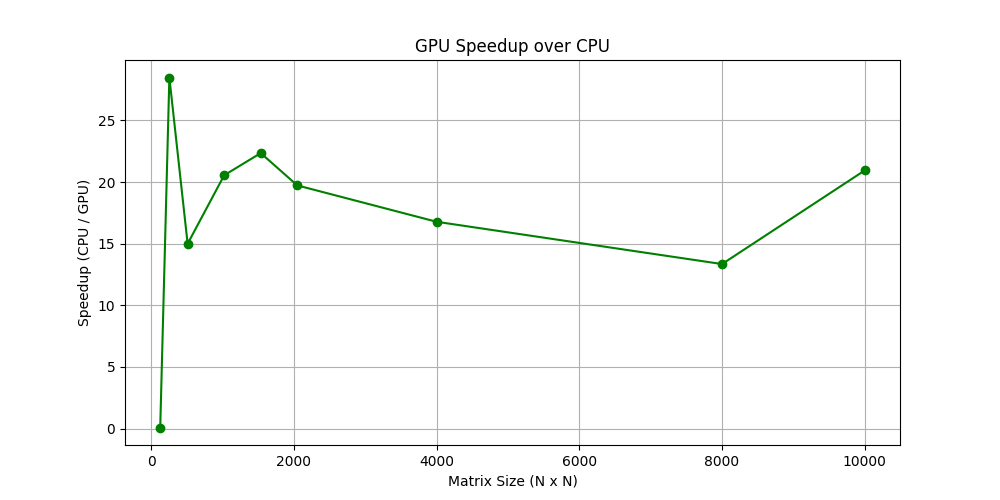
\includegraphics[width=0.92\textwidth]{speedup.png}
  \caption{GPU speedup ratio (CPU time / GPU time) across matrix sizes. The curve shows a sharp rise at small sizes (GPU parallelism kicks in), a plateau in the mid-range, a temporary dip at $n = 8000$ (memory bandwidth pressure), and a recovery at $n = 10000$.}
  \label{fig:speedup}
\end{figure}

% ═════════════════════════════════════════════════════════════════════════════
\section{Analysis and Discussion}

\subsection{Small Matrices: GPU Overhead Dominates ($n = 128$)}

At $n = 128$ the GPU is \textbf{slower} than the CPU (speedup $< 1$).  Launching a CUDA kernel, transferring control to the GPU, and synchronizing the device all incur fixed overhead in the range of milliseconds.  The actual computation ($128^3 \approx 2 \times 10^6$ FLOPs) is trivially small compared to this overhead, so the CPU finishes first.

\subsection{Rapid Rise in Speedup ($n = 256$--$1536$)}

Once the problem is large enough to saturate the GPU's streaming multiprocessors, speedup jumps sharply---peaking near \textbf{28$\times$} at $n = 256$ and stabilising around 20$\times$ through $n = 1536$.  The GPU executes thousands of independent multiply-accumulate operations in parallel, while the CPU is constrained to its core count and BLAS threading model.

\subsection{Mid-Range Plateau ($n = 2048$--$4000$)}

Speedup gradually decreases from $\approx 22\times$ to $\approx 17\times$ as the matrices grow past what fits comfortably in L2/L3 GPU cache.  Memory traffic begins to limit throughput on both platforms, though the GPU's high-bandwidth memory (HBM) maintains a clear advantage.
\clearpage
\subsection{Large Matrix Dip and Recovery ($n = 8000$--$10000$)}

At $n = 8000$ speedup drops to $\approx 13\times$.  A single $8000 \times 8000$ \texttt{float32} matrix consumes $\approx 244$ MB; holding three such matrices simultaneously pushes the GPU VRAM close to its limit, increasing eviction and re-transfer costs.

Interestingly, speedup \textbf{recovers} to $\approx 21\times$ at $n = 10000$.  A likely explanation is that the CPU suffers even more from its limited last-level cache at this scale, making the CPU-over-GPU penalty worse in absolute terms and thereby lifting the ratio.


% ═════════════════════════════════════════════════════════════════════════════
\section{Conclusion}

This experiment demonstrates quantitatively that GPU-accelerated matrix multiplication via CuPy offers substantial speedups over CPU-based NumPy for matrix sizes commonly encountered in engineering and machine learning workloads.  The speedup is not monotonic---GPU overhead dominates at tiny sizes, and memory pressure reduces efficiency at extreme sizes---but in the practically important range ($n \approx 1000$--$5000$), the GPU delivers a consistent \textbf{$15\times$--$22\times$} speedup.


\end{document}